%ullright document template
%default a4 one-sided article page setup
\documentclass[article, a4paper, oneside, 11pt]{memoir}

%the following three commands are necessary when using pdflatex
%(set input/output encoding)
\usepackage[utf8]{inputenc}
\usepackage[T1]{fontenc}
\usepackage{helvet}

%use sans serife font for body 
\renewcommand*\familydefault{\sfdefault}


%but with more tech-doc like margins
\setlrmarginsandblock{2.8cm}{2.8cm}{*}
\checkandfixthelayout

%for the german language
\usepackage[ngerman]{babel}

%including pictures
\usepackage{graphicx}
\graphicspath{{./figures/}}

%wrapping text around figures
\usepackage{wrapfig}

%provides symbols for shift, enter, etc.
\usepackage{keystroke}

%url handling
\usepackage{url}

%for code examples
\usepackage{listings}

%elaborate references
\usepackage[ngerman]{varioref}

%enables pdf linking and attributes
\usepackage{hyperref}
\hypersetup{
    colorlinks=true,%
    citecolor=black,%
    filecolor=black,%
    linkcolor=ullblue,%
    urlcolor=ullblue,%
    pdfauthor={ull.at},%
}

%removes page number from frontpage
\pagestyle{empty}

%header and footer images on every page
\usepackage{wallpaper}
\ULCornerWallPaper{1.0}{../../../ullCorePlugin/doc/manual/figures/header}
\LLCornerWallPaper{1.0}{../../../ullCorePlugin/doc/manual/figures/footer}

%Precise figure placement
% \usepackage{float}

%padding for fbox borders
%\setlength\fboxsep{0pt}

%color headlines
\usepackage{color}
\usepackage{titlesec}

\definecolor{ullblue}{rgb}{0.1, 0.42, 0.59}


\titleformat{\chapter}{\color{ullblue}\normalfont\huge\bfseries}{\thechapter}{0.75em}{\huge}

%each chapter on a new page
\let\stdchapter\chapter
\renewcommand*{\chapter}{\clearpage\stdchapter}

%each chapter title starts at the top of the page (reduce top margin)
\titlespacing{\chapter}{0pt}{-3em}{2em}

% Do not indent paragraphes but add newlines
\usepackage{parskip}
\setlength{\parindent}{0cm}
\setlength{\parskip}{2mm}


%memoir recommendation
\clubpenalty=10000
\widowpenalty=10000
\raggedbottom


\hypersetup{
    pdftitle={ullWiki Handbuch},%
    pdfsubject={ullright - ullWiki}
}

%%%%%%%%%%%%%%%%%%%%%%%%
% Document starts here %
%%%%%%%%%%%%%%%%%%%%%%%%


\begin{document}

\vspace*{3cm}
%move picture left/right
\begin{figure}[htp]
\centering

\includegraphics[width=0.5\textwidth]{softwarebox}
\end{figure}

\vspace{3cm}

%we do not use xelatex anymore
{%\fontspec[Scale=1.4, Color = DocBlue]{Ubuntu Bold}
\huge
\color{ullblue}
ullWiki – Wissensmanagement leicht gemacht
}

\vspace{1cm}

Ein Modul der ullright-Plattform -- \href{http://www.ullright.org}{www.ullright.org}

Online ausprobieren unter \href{http://demo.ullright.org}{demo.ullright.org}. 

Zuletzt geändert: 14.12.2011 -- Klemens Ullmann-Marx

\clearpage

\pagestyle{plain}

%\setcounter{page}{1}

%number and include in toc up until subsections
\setcounter{secnumdepth}{2}
\setcounter{tocdepth}{2}
\tableofcontents*

\clearpage


\chapter{Einführung}
ullWiki ist das Dokumentations- und Wissensmanagement-Modul der ullright Plattform.

Es zeichnet sich durch eine sehr einfache Bedienung aus, um Sie und Ihre Mitarbeiter optimal bei Dokumentations-Aufgaben und Wissensaustausch unterstützt werden. 

Unsere Kunden setzen ullWiki für vielfältige Aufgaben ein. Hier einige Beispiele:

\begin{itemize}
\item Dokumentation allgemein:

\begin{itemize}
\item Anleitungen, Prozessbeschreibungen, Notizen
\item Im IT-Bereich: Installationsanleitungen, Konfigurationen, HowTos
\end{itemize}

\item Problemlösungsdatenbank für Helpdesks in Verbindung mit dem ullFlow TroubleTicketing
\item Intranet: durch das einfache Verlinken von Seiten ist das ullWiki sogar als einfaches Intranet benutzbar.
\item Extranet: durch das Zugriffsrechtsystem können Sie bestimmte Dokumente auch für Kunden freigeben und so den Datenaustausch vereinfachen.
\end{itemize}

Die wichtigsten Funktionalitäten im Überblick:

\begin{itemize}
\item Eine WYSIWYG-Editor, der ohne HTML Kenntnisse die Erstellung formatierter Dokumente, ähnlich wie OpenOffice Writer oder MS Word erlaubt. Auch das Einfügen von Bildern oder Anhängen ist dadurch einfach möglich.
\item Suchfunktion: Ein einfaches Suchfeld durchsucht alle wichtigen Felder. Zusätzlich steht eine leistungsfähige Volltextsuche zur Verfügung.
\item Für jedes ullWiki-Dokument können Tags, also Schlagwörter vergeben werden. Dies erlaubt das schnelle Auffinden von Dokumenten und eine effiziente Kategorisierung.
\item Zugriffsebenen: Für jedes Dokument können Zugriffsrechte eingestellt werden. Diese erfolgern benutzerfreundlich über vordefinierte Zugriffsebenen.
\end{itemize}




\chapter{Startseite}

Jedes ullright Modul ist ähnlich aufgebaut damit Sie sich schnell zurechtfinden.

Die Startseite besteht aus drei Spalten (von links nach rechts) (Siehe Abbildung \vref{fig:index}):

\begin{itemize}
\item Aktionen
\item Suchfunktionen
\item Abfragen
\end{itemize}

\begin{figure}[htp]
\centering
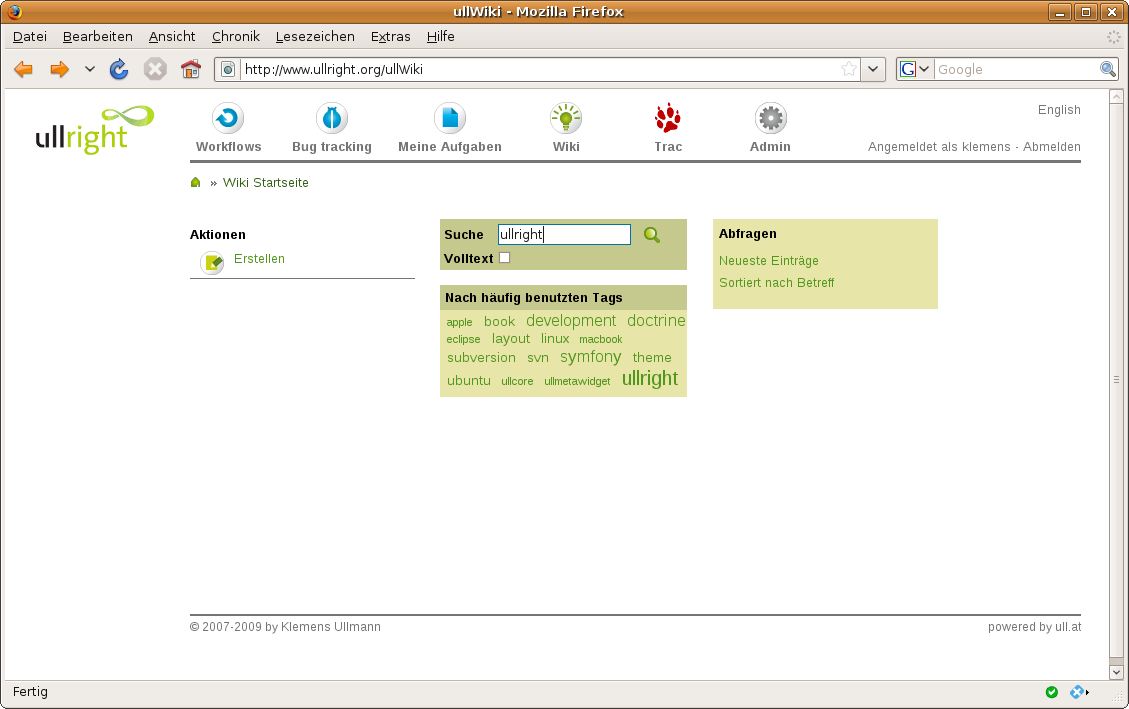
\includegraphics[width=0.9\textwidth]{index}
\caption{Startseite}
\label{fig:index}
\end{figure}

\section{Neues Dokument erstellen}
Häufig möchte man schnell einen Gedanken oder Einfall dokumentieren. Dafür ist natürlich der Punkt ein neues Dokument zu erstellen am wichtigsten. Falls Sie noch nicht in "`ullright"' angemeldet sind, werden sie praktischerweise sofort zur Anmeldemaske weitergeleitet. Auch nach der Anmeldung landen Sie nicht irgendwo, sondern direkt auf der Erstellungsseite.

\section{Suchfunktionen}
Geben Sie einfach jeglichen gewünschten Begriff in das Suchfeld ein. Wenn Sie auch den Text der Dokumente durchsuchen wollen, haken Sie bitte "`Volltext"' an. Die Suchfunktion sucht in den Feldern Id, Betreff und Tags.

Sie können Dokumente auch direkt anhand von Tags auswählen. Klicken Sie dazu einfach auf einen Tag und Sie erhalten eine Liste aller Dokumente für die dieses Tag vergeben wurde

\section{Abfragen}
Verwenden Sie die Abfragen um alle Einträge anzusehen. Individuelle Abfragen ergänzen wir Ihnen gerne auf Anfrage.

\section{Administration}
Verwalten Sie hier die Zugriffsrechte. Siehe Kapitel \vref{sec:admin} für Details.



\chapter{Ergebnisliste}
Auf der Ergebnislisten-Maske haben Sie alle wichtigen Funktionen zur Verfügung (Siehe Abbildung \vref{fig:list}):

\begin{itemize}
\item Neues Dokument erstellen
\item Suche
\item Ergebnislisten
\end{itemize}
Aus diesem Grund verlinkt ullright standardmäßig auf die Ergebnisliste des Wikis, und nicht auf die Startseite.

\begin{figure}[htp]
\centering

\includegraphics[width=0.9\textwidth]{list}
\caption{Ergebnisliste}
\label{fig:list}
\end{figure}


\section{Anzahl der Ergebnisse und Blättern}
Sie sehen die Anzahl der gefunden Dokumente, und welche Einträge gerade angezeigt werden. Standardmäßig werden 30 Einträge pro Seite angezeigt. Benutzen Sie die Funktion "`Blättern"' auf der rechten Seite um zur nächsten, oder einer beliebigen Seite der Ergebnisliste zu kommen.

\section{Liste}
Damit Sie die neuesten Einträge stets in Griffweite haben, sortiert die Ergebnisliste standardmäßig nach dem Aktualisierungsdatum. Sie finden also die zuletzt geänderten Dokumente ganz oben.

Klicken Sie auf eine der Spaltenüberschriften um nach dieser Spalte zu sortieren. Klicken Sie ein weiteres Mal um die Sortierung umzukehren.

Mittels der ersten beiden Symbole jeder Zeile können Sie einen Eintrag bearbeiten oder löschen.

Durch Klick auf den Betreff gelangen Sie zur Ansicht des Dokuments.

\section{Tipp: Die Browser Adresszeile als Kommandozeile}
Alle ullright Module unterstützen aktiv das sogenannte "`Deep Linking"'. Das bedeutet, daß alle wichtigen Parameter, wie zum Beispiel ein Suchbegriff, in der Adressleiste angeführt sind.

Sie können also jederzeit eine ullright Adresse als Bookmark (Favorit) speichern oder einer Kollegin per E-Mail schicken.

Beispiel: \url{http://www.ullright.org/ullWiki/list/filter[search]/openoffice}

Zeigt die Ergebnisliste für den Suchbegriff "`openoffice"'




\chapter{Erstellen und Bearbeiten}
Auch die Bearbeitungsseite präsentiert sich einfach und aufgeräumt (Siehe Abbildung \vref{fig:create-edit}).

Geben Sie einfach Betreff, Text, Tags und Zugriffsrecht an und Speichern Sie.

\begin{figure}[htp]
\centering
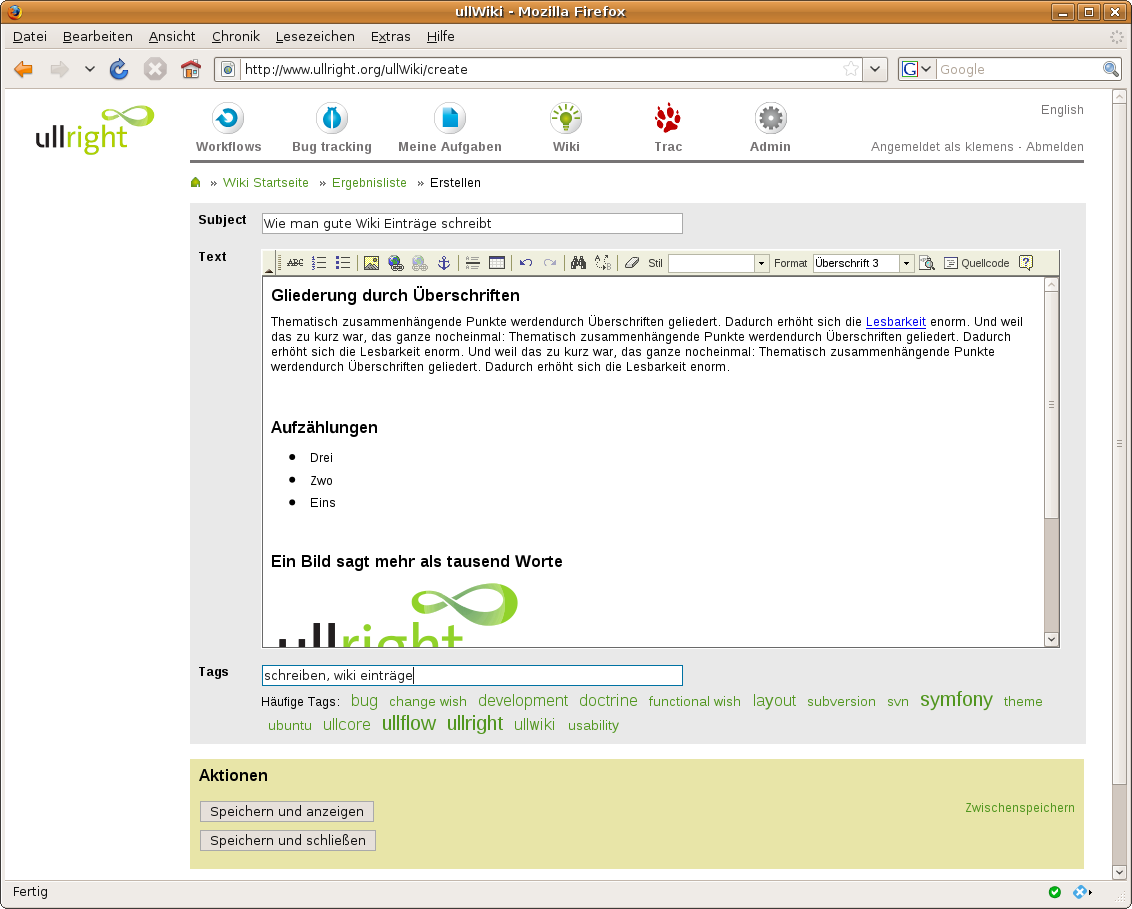
\includegraphics[width=0.9\textwidth]{create-edit}
\caption{Erstellen - Bearbeiten}
\label{fig:create-edit}
\end{figure}


\section{Text}
Viele Wikis verlangen nach HTML-Kenntnissen oder einer speziellen Syntax um den Text zu formatieren. ullWiki hingegen bietet einen komfortablen Editor, der ähnlich wie OpenOffice Writer oder MS Word funktioniert. Auch das Einfügen von Bildern oder Anhängen ist, wie weiter unten beschrieben, leicht möglich.

Details zur Bedienung des Editors erfahren Sie im Kapitel \vref{sec:editor}.


\section{Tags}
Vergeben Sie sinnvolle Schlagworte (=Tags) um das Dokument zu kategorisieren und die Suche zu vereinfachen. 

Geben Sie einen neues Schlagwort ein und klicken Sie auf "`Hinzufügen, oder klicken Sie auf ein bereits vorhandenes Schlagwort in der "'Tag-Cloud"`.

Ein Klick auf das Papierkorb-Symbol entfernt ein gewähltes Schlagwort.



\section{Zugriffsebene}
Viele Wikis bieten keine oder komplizierte Zugriffsrechts-Mechanismen die mitunter umständlich zu bedienen sind. Häufig müssen Sie hierbei für jedes Dokument erneut auswählen welche Benutzer und Gruppen Zugriff darauf haben sollen.

Nicht so bei ullWiki: Wir stellen eine erweiterbare Liste an vordefinierten Zugriffsebenen zur Verfügung. Jede Zugriffsebene kann im Hintergrund komplexe Berechtigungen enthalten.

Wählen Sie nun also einfach die gewünschte Zugriffsebene für das aktuelle Dokument aus der Liste aus.

Standardmäßig finden Sie folgende Zugriffsebenen in der Liste:

\begin{itemize}
\item Öffentlich lesbar – Jeder kann lesen und angemeldete Benutzer können bearbeiten.
\item Für angemeldete Benutzer lesbar – Nur angemeldete Benutzer können lesen und bearbeiten.
\end{itemize}
Die Liste der Zugriffsrechte kann beliebig erweitert werden – Siehe Kapitel \vref{sec:admin}.

\section{Speichern}
Damit Sie möglichst effizient Arbeiten können, stellen wir mehrere Buttons zum Speichern zur Verfügung. So sparen Sie zum Beispiel bei "`Zwischenspeichern"' mehrere Klicks im Vergleich zu anderen Wikis, die nur einen "`Speichern"' Button bieten, und Sie zum weiter-bearbeiten erneut zur Bearbeitungsseite navigieren müssen.

\begin{itemize}
\item Speichern und anzeigen: Speichert das Dokument und zeigt die Ansichtsseite
\item Speichern und schließen: Speichert das Dokument und kehrt zurück zur Ergebnisliste
\item Zwischenspeichern: Speichert aber bleibt auf der Bearbeitungsseite
\end{itemize}

\section{Automatisches Speichern}
Während Sie ein Wiki-Dokument editieren speichert das System regelmäßig im Hintergrund Ihre Änderungen. Sie können nebenbei wie gewohnt arbeiten. Der Vorgang des Speicherns wird durch die Einblendung \emph{Automatisches Speichern ...} gekennzeichnet. Im Erfolgsfall erscheint \emph{Gespeichert}. 

Falls beim Automatischen Speichern ein Fehler auftritt wird eine entsprechende Meldung eingeblendet. Zusätzlich erscheint ein Button, der die Möglichkeit bietet, die Gründe für das Fehlschlagen des Speichervorgangs anzuzeigen.

\textbf{Achtung:} Das Automatische Speichern wird nur bei der Bearbeitung eines Wiki-Dokuments automatisch aktiviert. Falls Sie ein neues Dokument erstellen müssen Sie es erstmalig \emph{Zwischenspeichern} um das Automatische Speichern zu aktivieren. 


\chapter{Text bearbeiten mit dem "`WYSIWYG"' Editor}
\label{sec:editor}

"`WYSIWYG"' steht für "`What you see is what you get"',  also dass man schon bei der Eingabe sieht wie der Text letztendlich aussehen wird.

Die angezeigten Formatierungs-Möglichkeiten können sich je nach Konfiguration und Editor-Version von Ihrer Installation unterscheiden.

\begin{figure}[htp]
\centering
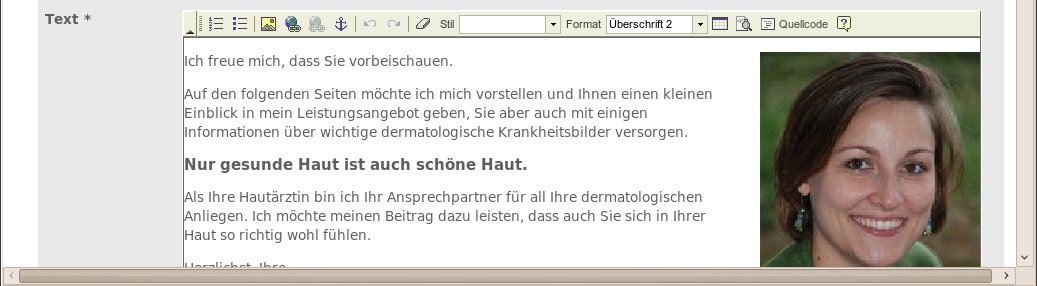
\includegraphics[width=0.9\textwidth]{../../../ullCorePlugin/doc/manual/figures/editor}
\caption{WYSIWYG-Editor}
\label{fig:editor}
\end{figure}

\section{Text schreiben}

Geben Sie wie von anderen Texteditoren gewohnt den Text ein.

Tipp: $\Enter$ erzeugt einen neuen Paragrafen, also einen Textblock mit einer Leerzeile dahinter. Einen einfachen Zeilenumbruch erreichen Sie mit $\Shift + \Enter$.

\section{Text formatieren}

Markieren Sie den gewünschten Text und wählen Sie aus der Editor-Menüleiste die gewünschte Auszeichnung.

Bitte beachten Sie, dass die von uns ausgewählten
Formatierungsmöglichkeiten nach semantischen Gesichtspunkten ausgewählt
wurden. Sie finden also nur „logische“ Auszeichnungen wie zum Beispiel
„wichtig“ oder „Überschrift“, und keine rein optischen
Formatierungsmöglichkeiten wie Farben oder Schriftgrößen. Somit werden
saubere und zukunftssichere Texte gewährleistet. (Stichwort "`semantic
Web"')

Die wichtigsten Formatierungen (von links nach rechts):

\begin{itemize}
\item Nummerierte Liste
\item Liste mit Aufzählungszeichen
\item Stile: "`Important"' -- also "`Wichtig"' wird fett angezeigt
\item Format: "`Überschrift"'
\end{itemize}


\section{Bild einfügen}

\begin{itemize}
\item Setzten Sie den Cursor an die gewünschte Stelle im Text
\item Klicken Sie auf das Bildsymbol 
\includegraphics[height=5mm]{../../../ullCorePlugin/doc/manual/figures/image_icon}
\item Wählen Sie "`Server durchsuchen"'
\item Wählen oder erstellen Sie gegebenenfalls einen neuen Ordner um eine ordentliche Struktur Ihrer Daten zu gewährleisten
\item Wenn Sie ein neues Bild hochladen möchten klicken Sie auf "`Durchsuchen"' und wählen Sie eine Bilddatei von Ihrem Computer aus.
\item Vergessen Sie nicht danach auf "`Upload"' zu klicken
\item Wählen Sie nun ein Bild aus der Liste durch anklicken.
\item Klicken Sie auf "`OK"'
\end{itemize}

\section{Bildeigenschaften ändern}

Klicken Sie mit der rechten Maustaste auf das Bild und wählen Sie "`Bildeigenschaften"'.

Im folgenden werden die wichtigsten Eigenschaften erklärt:

\subsection{Reiter "`Bild-Info"'}

\begin{itemize}
\item Breite / Höhe - Wählen Sie die gewünschte Größe des Bildes in Pixel. Bitte beachten Sie, dass Bilder bereits vor dem Hochladen mit einem Grafikprogramm auf die endgültige Größe skaliert werden sollten
\item Ausrichtung - Wählen Sie "`Links"' oder "`Rechts"' wenn der Text das Bild umfließen soll.
\end{itemize}

\subsection{Reiter "`Erweitert"'}

Wenn Sie das Bild vom Text umfließen lassen ist häufig auf gewissen Seiten des Bildes ein Abstand erwünscht.
Dieser Abstand kann im Feld "`Style"' angegeben werden. Beispiel für einen Abstand links und unten: "`margin-left: 1.5em; margin-bottom: 1.5em;"'


\section{Link erstellen}

Normale Webadressen und E-Mailadressen werden in der normalen Ansicht für die Besucher der Webseite automatisch verlinkt.

Beispiele:

\begin{itemize}
\item www.ullright.org
\item http://ull.at
\item office@ull.at
\end{itemize}

Möchten Sie hingegen gewisse Wörter im Text verlinken markieren Sie die Wörter und klicken Sie auf das Linksymbol 
\includegraphics[height=5mm]{../../../ullCorePlugin/doc/manual/figures/link_icon} (blau-grüne Erdkugel).

\subsection{Link zu einer Internetadresse (URL)}
Geben Sie bei "`URL"' die gewünschte Adresse ein. Beispiel: \url{http://www.ullright.org}

Bei Links zu Internetseiten empfiehlt sich die Seite in einem neuen Browserfenster zu öffnen. Wählen Sie hierzu im Reiter "`Zielseite"' "`Neues Fenster (\_blank)"'.

Zusätzlich empfehlen wir einen solchen Link durch das Symbol für "`Externe Seite"' zu kennzeichen. Schreiben Sie dazu im Reiter "`Erweitert"' die Anweisung "`link\_external"' in das Feld "`Stylesheet Klasse"'.

\subsection{Link zu einer anderen CMS-Seite}

Öffnen Sie die Zielseite in einem neuen Browsertab oder -fenster und kopieren Sie die URL aus der Adressleiste.

Beispiel: \url{http://www.ull.at/ullCms/show/kontakt}

Geben Sie nun bei "`URL"' die gekürzte Adresse startend mit den Schrägstrich nach dem Domänennamen ein.

Beispiel: \url{/ullCms/show/kontakt}

\subsection{E-Mail Link}

Wählen Sie bei "`Link-Typ"' E-Mail und geben Sie die gewünschte E-Mailadresse ein.



\section{Datei hochladen}
\label{sec:upload_file}

Das Hochladen einer Datei funktioniert wie eine Mischung aus Link- und Bildeinfügen.

\begin{itemize}
\item Markieren Sie die Wörter die mit der Datei verlinkt werden sollen
\item Klicken Sie auf das Linksymbol 
\includegraphics[height=5mm]{../../../ullCorePlugin/doc/manual/figures/link_icon}
\item Wählen Sie „Server durchsuchen“
\item Wählen oder erstellen Sie gegebenenfalls einen neuen Ordner um eine ordentliche Struktur Ihrer Daten zu gewährleisten
\item Wenn Sie eine neue Datei hochladen möchten klicken Sie auf "`Durchsuchen"' und wählen Sie eine Datei von Ihrem Computer aus
\item Vergessen Sie nicht danach auf "`Upload"' zu klicken
\item Wählen Sie nun die Datei aus der Liste durch anklicken
\item Klicken Sie auf "`OK"'
\end{itemize}


\section{Tip für PDF-Dateien}

Auf vielen PCs wird bei einem Klick auf den Link zu einer PDF-Datei das PDF direkt im Browserfenster geöffnet. Besuchern passiert es dann häufig, dass sie nach dem Lesen das Fenster oder Tab einfach schließen, und somit auch Ihre Website verlassen.

Um diesem unerwünschten Verhalten vorzubeugen empfiehlt sich ein PDF in einem Pop-up Fenster zu öffnen:

\begin{itemize}
\item Verlinken Sie eine PDF-Datei wie im Kapitel \vref{sec:upload_file} beschrieben
\item Klicken Sie mit der rechten Maustaste auf den Link zur PDF-Datei und wählen Sie "`Link editieren"'
\item Im Reiter "`Zielseite"' wählen Sie nun "`Pop-up Fenster"'
\item Haken Sie die Felder "`Vergrößerbar"', "`Adress-Leiste"', "`Menüleiste"' und "`Rollbalken"' an.
\item Schließen Sie den Vorgang mit "`OK"' ab.
\end{itemize}



\chapter{Ansicht}
Durch Klick auf den Betreff in der Ergebnisliste wird das Dokument im Ansichtsmodus geladen (Siehe Abbildung \vref{fig:show}).

Mittels der ersten beiden Symbole "`Stift"' und "Papierkorb"' können Sie einen Eintrag bearbeiten oder löschen.

Am Ende des Dokuments erfahren Sie Detailinformationen zum Dokument, also wer und wann es erstellt hat, und wer und wann es aktualisiert hat.

\begin{figure}[htp]
\centering
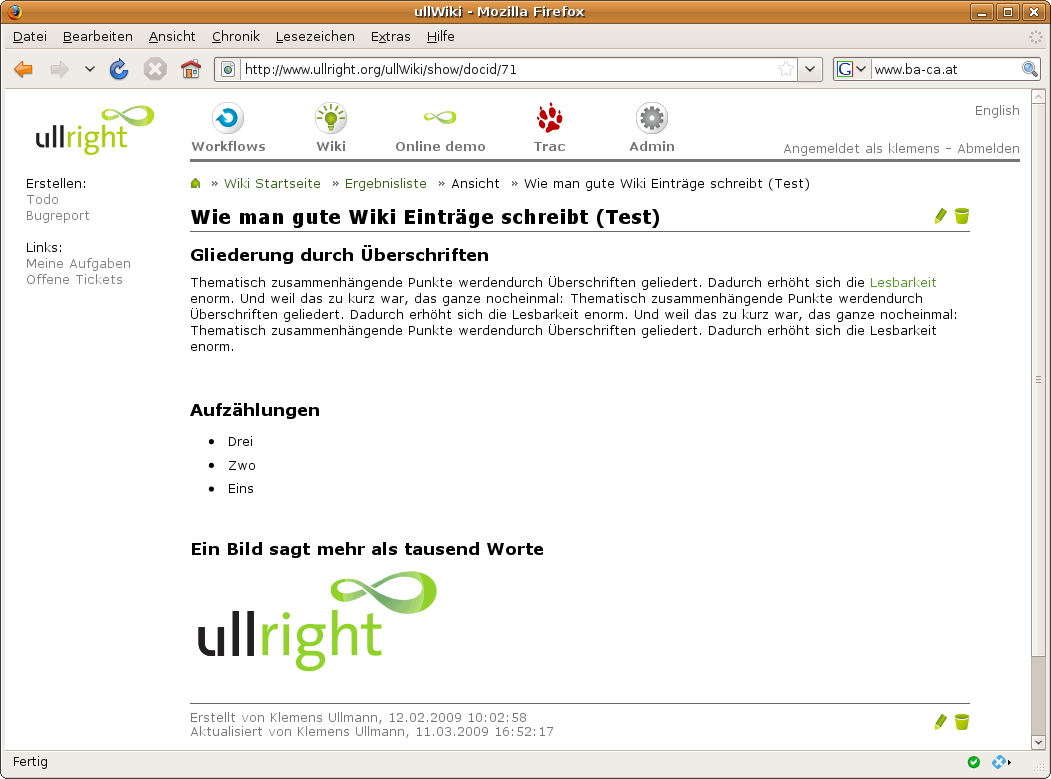
\includegraphics[width=0.9\textwidth]{show}
\caption{Ansicht eines Eintrags}
\label{fig:show}
\end{figure}

%\clearpage


\chapter{Administration - Zugriffrechte}
\label{sec:admin}

Melden Sie sich als Benutzer mit Adminstrator-Rechten an und navigieren Sie zur ullWiki-Startseite. Dort finden Sie die folgenden Funktionen im Bereich "`Administration"'.

ullWiki bietet ein sehr flexibles und dennoch einfach zu bedienendes Zugriffsrechtsystem.

Zugriffsrechte sind in sogenannte \emph{Zugriffsebenen} organisiert. Diese tragen einen sprechenden Namen und sind beim Bearbeiten eines Wiki-Dokuments schnell und einfach auszuwählen.

Beispiele: 

\begin{itemize}
\item "`Öffentlich lesbar"'
\item "`Einkauf"' - Nur für diese Abteilung
\item "`Kunde XYZ"' - Nur für einen Kunden 
\end{itemize}


\section{Zugriffsebenen verwalten}
Wählen Sie auf der Wiki-Startseite den Punkt "`Administration - Verwalte Zugriffsebenen"'.

Sie sehen nun eine Liste der aktuell angelegten Zugriffsebenen.

Klicken Sie auf "`Erstellen"' um einen neue Ebenen anzulegen oder auf das Stiftsymbol um den Namen einer Ebenen zu ändern.

Speichen Sie mit "`Speichern und zurück zur Liste"'.



\section{Zugriffsrechte verwalten}
Unter diesem Punkt legen Sie nun für jede Zugriffsebene genau fest welche Gruppe lesen und/oder schreiben darf.

Wählen Sie auf der Wiki-Startseite den Punkt "`Administration - Verwalte Zugriffsrechte"'.
Sie sehen nun eine Liste der aktuell angelegten Zugriffsrechte.

Jedes Zugriffsrecht stellt eine Zuordnungnach dem Scheme "`Gruppe"' - "`Privileg"' - "`Zugriffsebene"' dar.

Beispiel: Gruppe "`Einkauf"' darf Einträge lesen der Zugriffsebene "`Einkauf"'.

Erstellen Sie eine neue Zuordnung über "`Erstellen"'.

Löschen Sie eine Zuordnung mit dem Papierkorbsymbol.

Bearbeiten lässt sich eine Zuordnung mit dem Stiftsymbol.


\section{Praktisches Beispiel}

Sie möchten einen Wiki-Eintrag für einen oder mehrere Mitarbeiter eines Kunden freigeben.

\subsection{Gruppe anlegen}
Die Vergabe der Rechte funktioniert über Gruppen. Daher muss, falls nicht bereits vorhanden, eine Gruppe für den Kunden angelegt werden:

\begin{itemize}
\item Menüpunkt "`Admin"' aufrufen
\item "`Verwalte Gruppen"'
\item "`Erstellen"'
\item Den gewünschten Gruppennamen bei "`Anzeigename"' eintragen. Z.B. "`Kunde XYZ"'.
\item "`Speichern und zurück zur Liste"'
\end{itemize}

\subsection{Benutzer anlegen}
Falls die Mitarbeiter noch nicht als Benutzer angelegt sind:

\begin{itemize}
\item Menüpunkt "`Admin"' aufrufen
\item "`Erstelle Benutzer"'
\item Daten eingeben - zumindest Vorname, Nachname, Benutzername und E-Mailadresse
\item Bei "`Gruppenmitgliedschaften"' die oben erstellte Gruppe auswählen
\item "`Speichern und zurück zur Liste"'
\end{itemize}

Falls die Mitarbeiter bereits angelegt sind müssen Sie noch Mitglieder der Gruppe werden:
\begin{itemize}
\item Menüpunkt "`Admin"' aufrufen
\item Über die Benutzerauswahl die gewünschte Person wählen
\item Bei "`Gruppenmitgliedschaften"' die oben erstellte Gruppe auswählen
\item "`Speichern und zurück zur Liste"'
\end{itemize}

\subsection{Wiki-Zugriffsebene erstellen}
\begin{itemize}
 \item Die ullWiki-Startseite aufrufen
 \item "`Verwalte Zugriffsebenen"'
 \item "`Erstellen"'
 \item Eine sprechende Bezeichnung eingeben. Z.B. "`Kunde XYZ"'
 \item "`Speichern und zurück zur Liste"'
\end{itemize}

\subsection{Wiki-Zugriffsrechte einstellen}
Zuletzt noch die tatsächlichen Zugriffsrechte einstellen:
\begin{itemize}
 \item Die ullWiki-Startseite aufrufen
 \item "`Verwalte Zugriffsrechte"'
 \item "`Erstellen"'
    \begin{itemize}
      \item Gruppe: "`Kunde XYZ"'
      \item Privileg: "`read"' (lesen)
      \item Zugriffsrecht: "`Kunde XYZ"'
      \item "`Speichern und neu"'
    \end{itemize}
    \begin{itemize}
      \item Gruppe: z.B. "`MasterAdmins"' oder wie gewünscht
      \item Privileg: "`write"' (schreiben)
      \item Zugriffsrecht: "`Kunde XYZ"'
      \item "`Speichern und zurück zur Liste"'
    \end{itemize}
\end{itemize}

Fertig! Wählen Sie nun bei Ihrem Wiki-Dokumente die neue Zugriffsebene und senden Sie den entsprechenden Personen Username, Passwort und einen Link zum Dokument (Ansichtsmodus und dort die Internetadresse kopieren).

\end{document}
